\section{Distributed Processing of Spatial Algorithms}
\label{sec:spatial_dist}		
A number of structures have been proposed for handling multi-dimensional spatial data, such as: 
KD-Tree \cite{bentley1975multidimensional}, Hilbert R-Tree \cite{kamel1994hilbert} and R-Tree \cite{guttman1984r}.
The R-Tree has been widely used to index the datasets on GIS databases and it has been used as an index data structure in this work.

A R-Tree is a height-balanced tree similar to a B-Tree \cite{comer1979ubiquitous} with index records in its leaf nodes containing pointers to data objects. 
The key idea of the data structure is to group nearby objects and represent them with their minimum bounding rectangle (MBR) in the next higher level of the tree. 

Figure \ref{fig:rtree} illustrates the hierarchical structure of a R-Tree with a root node, internal nodes ($N1...2 \subset N3...6$) and leaves ($N3...6 \subset a...h$). 
Every internal node contains a set of rectangles and pointers to the corresponding child node and every leaf node contains the rectangles of spatial objects.

The Figure \ref{fig:rtree-space} shows MBRs grouping spatial objects of $a...h$ in sets by their co-location. 
The Figure \ref{fig:rtree-index} illustrates the R-Tree representation. Each node stores at most $M$ and at least $m \leq M/2$ entries \cite{guttman1984r}. 
Our work uses the formula for $M$ value calculation presented in \cite{dedsi}.

\begin{figure}[h]
  \centering
  \subfigure[R-Tree index]
  {
  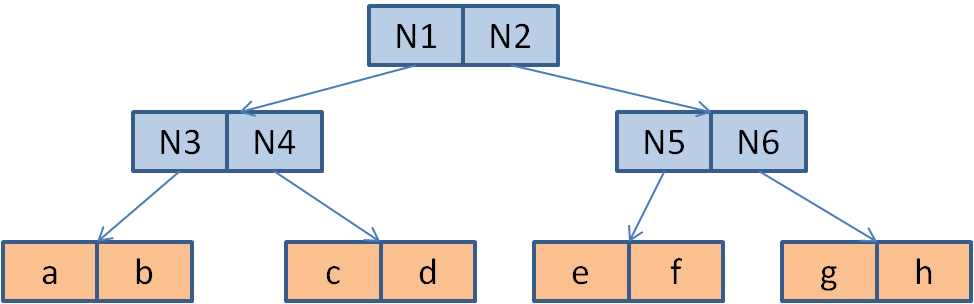
\includegraphics[width=0.45\textwidth]{rtree}
  \label{fig:rtree-index}
  } \qquad
  \subfigure[Geographic space]
  {
  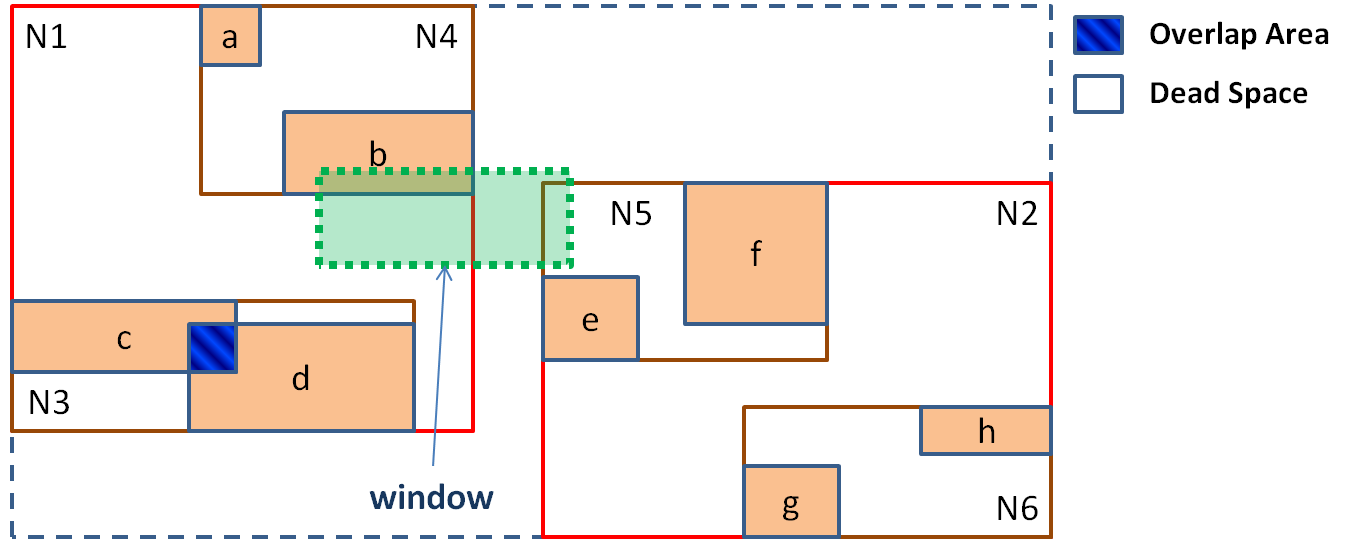
\includegraphics[width=0.45\textwidth]{rtree-space}
  \label{fig:rtree-space}
  }
  \caption{R-Tree Structure}
  \label{fig:rtree}
\end{figure}

The Window Query is one of major query algorithms in R-Tree.
The search starts from the root node of the tree and the input is a search rectangle (Query box). 
For each rectangle in a node, it has to be decided either it overlaps the search rectangle or not. If yes, the corresponding child node has to be searched also. 

Searching is done recursively until all overlapping nodes have been traversed. 
When a leaf node is reached, the contained bounding boxes (rectangles) are tested against the search rectangle 
and the objects that intersects with the search rectangle are returned.

In Figure \ref{fig:rtree}, the search starts on root node, where the window intersects with nodes $N1$ and $N2$. Then, the algorithm analyzes node $N1$, 
which only $N4$ intersects with the window. Analyzing node $N4$, the algorithm returns the spatial object namely $'b'$, that is the single object that intersects the window.

In node $N2$, we do not have any entry intersecting with the window due to the dead space. 
In other words, the window intersects with a space, which does not contain any data.
The dead space should be minimized to improve the query performance, since decisions which paths have to be traversed can be taken on higher levels. 

The overlapping area between rectangles should be minimized as well, as it degrades the performance of R-Tree \cite{beckmann1990r}. 
Less overlapping reduces the amount of sub-trees accessed during r-tree traversal. The area between c and d in Figure \ref{fig:rtree} is an example of overlapping.

\subsection{DistGeo: A Platform of Distributed Spatial Operations for Geoprocessing}
\label{sub:dist_geo}	

DistGeo is a platform to process spatial operations in a cluster of computers (Figure \ref{fig:dist}). 
It is based on a shared-nothing architecture, which the nodes do not share CPU, hard disk and memory and the communication relies on message exchange. 
Figure \ref{fig: Figure 3} depicts DistGeo platform based on peer-to-peer model presented as a ring topology. 
It is divided in ranges of keys, which are managed for each server of the cluster. In order to a server join the ring it must be assigned a range first.

The range of keys are known by each server in the cluster using a Distributed Hash Table (DHT) to store the mapping of the keys to servers. 
For instance, in a ring representation, whose key set start with 0 to 100, if we have 4 nodes in the cluster, the division could be done as shown below: 
a) 0-25, b) 25-50, c) 50-75 e d) 75-100. If we want to search for one object with key 34, we certainly should look on the server 2.

\begin{figure}[h]
  \centering
  \subfigure[DistGeo Architecture]
  {
  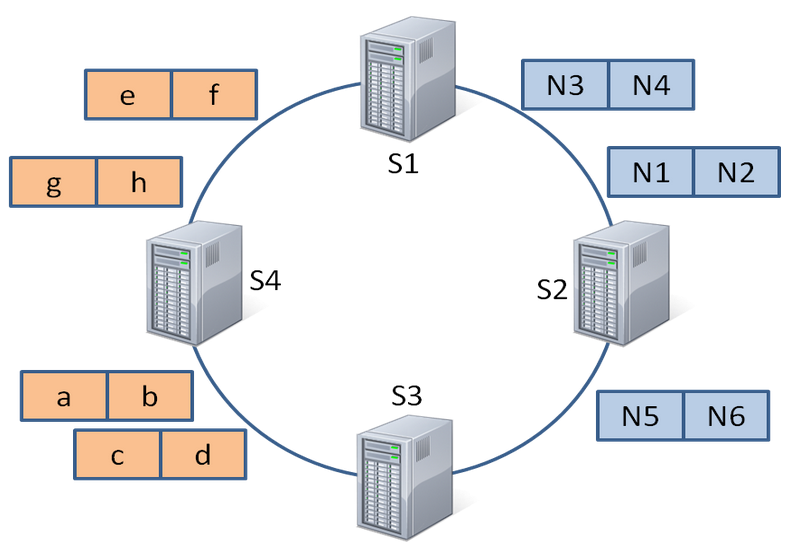
\includegraphics[width=0.45\textwidth]{figure3.png}
  \label{fig: Figure 3}
  } \qquad
  \subfigure[R-Tree Partitioning in DistGeo]
  {
  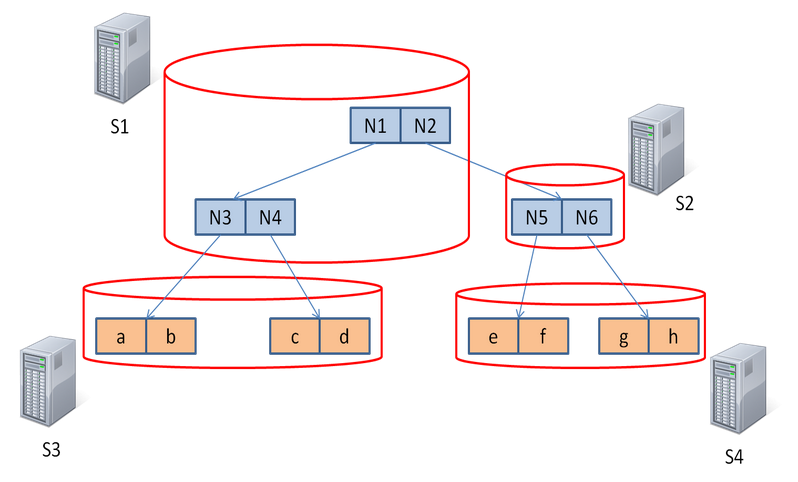
\includegraphics[width=0.45\textwidth]{r-tree-partiotioning.png}
  \label{fig:partitioning}
  }
  \caption{DistGeo Platform}
  \label{fig:dist}
\end{figure}
	
Every replica of an object is equally important, in other words, there is not a master replica. Read and write operations may be performed in any server of the cluster. 
When a request is made to a cluster's server, it becomes the coordinator of the operation requested by the client. 
The coordinator works as a proxy between the client and the cluster servers. 
	
DistGeo uses the Gossip protocol \cite{demers1987epidemic}, which every cluster server exchanges information 
among themselves for everyone knows the status of each server. 
In the Gossip protocol every second a message is exchanged among three servers in the cluster, 
consequently every cluster's server have knowledge of each other. 

Figure \ref{fig:partitioning} illustrates the structure of a Distributed R-Tree in a cluster. 
The partitioning it is performed grouping the servers in cluster and creating the indexes according to the R-Tree structure. 
The lines in Figure \ref{fig:partitioning} show the need for message exchange to reach the sub-trees during the algorithm processing. 

Insertions and searching in a distributed R-Tree are similar to the non-distributed version, except for: i) The need of message exchange to access the distributed partitions and
ii) Concurrency control and consistency due to the parallel processing in the cluster. Both were implemented on DistGeo platform.

The distributed index has been built according to the taxonomy defined in \cite{an1999storing}, as follows: i) Allocation Unit: block - A partition is created for every R-Tree node; 
ii) Allocation Frequency: overflow - In the insert process, new partitions are created when a node in the tree needs to split; 
iii) Distribution Policy: balanced - To keep the tree balanced the partitions are distributed among the cluster servers.
	
Reliability and fault-tolerance were implemented on DistGeo storing the R-Tree nodes in multiple servers in the cluster. 
The DistGeo uses Apache Cassandra \cite{cassandra1apache} database to store the distributed R-Tree index nodes on cluster servers.
Each R-Tree node N receives a key, which is used to store the node in a server S responsible for ring range, replicating the node N to the next two servers in S (clockwise). 
If a message is sent to N, is selected one of the servers that store a replica of N.
The query requests are always sent to one of the cluster's server that stores the root node of the R-tree. 

Some optimizations proposed in \cite{beckmann1990r} to reduce the overlapping and the dead area were adapted and implemented on DistGeo. 
Reducing the overlapping and dead area minimizes the number of messages exchange in network on search algorithms because the query accesses less nodes during the tree traversal (see Section \ref{sec:spatial_dist}). 
This work implements a new distributed debug algorithm of the R-Tree index (RDebug) that helps to reduce the overlap and dead area.
We cover the RDebug algorithm in more details in Section \ref{sec:rdebug}.